\documentclass[aspectratio=169,11pt]{beamer}
\usetheme{Madrid}
\usecolortheme{default}
\usepackage{xeCJK}
\setCJKmainfont{Noto Sans CJK JP}
\setCJKsansfont{Noto Sans CJK JP}
\usepackage{tikz}
\usetikzlibrary{positioning}
\usepackage{booktabs}
\usepackage{xcolor}
\setbeamertemplate{navigation symbols}{}
\setbeamertemplate{footline}[frame number]
\definecolor{TCUBlue}{RGB}{20,64,120}
\setbeamercolor{structure}{fg=TCUBlue}
\setbeamercolor{frametitle}{fg=white,bg=TCUBlue}
\setbeamerfont{frametitle}{size=\large,series=\bfseries}
\newcommand{\code}[1]{\texttt{\detokenize{#1}}}
\title{Small-PCAP Analysis-First}
\subtitle{小さなPCAPでpacket / flow / burstに親しむ}
\author{B3 Case Study 2026}
\date{}
\begin{document}
\begin{frame}\titlepage\end{frame}
\begin{frame}{A1: 最初は「研究対象」に親しむ}
\begin{block}{今日の目的}
PCAPを巨大データとしてではなく、まず観測されたpacketの列として触る。
\end{block}
\begin{itemize}
\item 小さなPCAPなら、手で追える。
\item Pythonからfieldを取り出せる。
\item PacketRecord, flow, burstの意味を確認できる。
\end{itemize}
\vfill
\centering\Large まずは小さなPCAPを「見て・触って・説明する」。
\end{frame}
\begin{frame}{A2: 二本のレール}
\centering
\begin{tikzpicture}[node distance=0.75cm, every node/.style={font=\small}]
\tikzstyle{box}=[draw, rounded corners, align=center, minimum width=4.3cm, minimum height=0.65cm]
\node[box] (l1) {Analysis-first\\小PCAPで親しむ};
\node[box, below=of l1] (l2) {packet / field};
\node[box, below=of l2] (l3) {flow / burst};
\node[box, right=2.2cm of l1] (r1) {Scale rail\\少し大きくする};
\node[box, below=of r1] (r2) {Scaling Wall};
\node[box, below=of r2] (r3) {streaming design};
\draw[->, thick] (l1)--(l2); \draw[->, thick] (l2)--(l3);
\draw[->, thick] (r1)--(r2); \draw[->, thick] (r2)--(r3);
\draw[->, thick] (l3.east)--(r2.west);
\end{tikzpicture}
\end{frame}
\begin{frame}{A3: PCAPを見るときの語彙}
\begin{itemize}
\item capture: packetを記録したファイル
\item packet: 時刻を持つ観測単位
\item header field: IP, port, protocol, lengthなど
\item derived field: 後から計算したIAT, direction, flow keyなど
\end{itemize}
\vfill
\begin{block}{問い}
これはPCAPから直接観測した値か？それとも自分たちが作った値か？
\end{block}
\end{frame}
\begin{frame}{A4: Python library-like path}
\begin{block}{最初は便利さを優先}
小さいPCAPでは、まずpacketを一つずつ取り出してfieldを見る。
\end{block}
\begin{itemize}
\item 必須path: repository内の小さなreader
\item optional: Scapy等が使える環境ではside-by-sideで眺めてもよい
\item 採点・比較の境界はPacketRecordにそろえる
\end{itemize}
\vfill
\code{python -m labs.lab0_pcap.demo}
\end{frame}
\begin{frame}{A5: field policyを作る}
\small
\begin{tabular}{p{0.25\textwidth}p{0.25\textwidth}p{0.38\textwidth}}
\toprule
Field & 観察/派生 & 注意 \\
\midrule
timestamp & observed & 差分が重要になることが多い \\
src/dst IP & observed & directionを定義する材料 \\
port & observed & TCP/UDP以外では無い場合もある \\
packet length & observed policy & L3 bytesかframe bytesかを明記 \\
payload length & derived from headers & 0でも意味がある \\
\bottomrule
\end{tabular}
\vfill
\centering\textbf{fieldを選ぶことは、情報を捨てることでもある。}
\end{frame}
\begin{frame}{A6: PacketRecord contractの始まり}
\centering
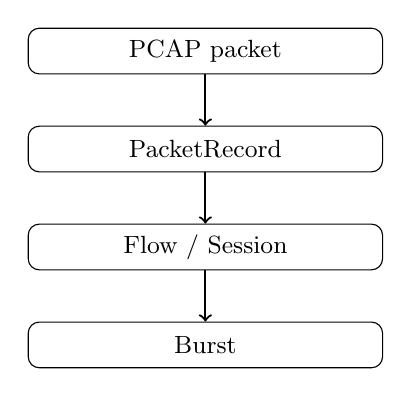
\begin{tikzpicture}[node distance=0.65cm, every node/.style={font=\small}]
\tikzstyle{box}=[draw, rounded corners, align=center, minimum width=4.5cm, minimum height=0.58cm]
\node[box] (p) {PCAP packet};
\node[box, below=of p] (r) {PacketRecord};
\node[box, below=of r] (f) {Flow / Session};
\node[box, below=of f] (b) {Burst};
\draw[->, thick] (p)--(r); \draw[->, thick] (r)--(f); \draw[->, thick] (f)--(b);
\end{tikzpicture}
\vfill
PacketRecordは全情報ではない。以後のrepresentation pipelineへの共通入口である。
\end{frame}
\begin{frame}{A7: packetからflow/burstへ}
\begin{itemize}
\item flow keyをどう定義するか？
\item A→BとB→Aを同じflowに入れるか？
\item session timeoutはいくつか？
\item burst boundaryはdirection changeか、time gapか？
\end{itemize}
\vfill
\begin{block}{小PCAPの利点}
手計算とコード出力を照合できる。抽象化の意味を見失いにくい。
\end{block}
\end{frame}
\begin{frame}{A8: 次の問いへ}
\centering
\Large 小さいPCAPなら、分かりやすく、楽しい。\\[1em]
\textbf{では、少し大きくしたら？}
\vfill
\normalsize
次は同じanalysis-first pathで、時間とメモリを測る。
\end{frame}
\end{document}
